\section{Datos}

Los datos empleados en este proyecto fueron obtenidos de \href{http://insideairbnb.com/}{Inside Airbnb}.

Inside Airbnb es un proyecto independiente querecopila y analiza datos procedentes de diversas ciudades alrededor del mundo que forman parte de la plataforma Airbnb. Fue creado con el objetivo de brindar transparencia y comprensión sobre el impacto de Airbnb en los mercados de alquiler a corto plazo. Inside Airbnb recopila datos públicos de las listas de Airbnb, como información sobre las propiedades, los anfitriones y la disponibilidad de alojamiento. Estos datos se utilizan para crear conjuntos de datos estructurados que permiten realizar análisis y visualizaciones detalladas sobre la oferta de alojamiento en cada ciudad.\\

Los datos utilizados en este estudio están disponibles en el enlace: \href{http://insideairbnb.com/get-the-data/}{http://insideairbnb.com/get-the-data/}.\\
Adicionalmente, es posible explorar una representación interactiva de los datos en la sección "Explorar datos", donde se presenta un mapa de Málaga a través de \ \href{http://insideairbnb.com/malaga/}{http://insideairbnb.com/malaga/}. Esta herramienta brinda una síntesis informativa sobre diversos aspectos de los datos relativos a Airbnb en la ciudad.
\begin{itemize}
  \item \textbf{Tipo de habitación}: Muestra el porcentaje de diferentes tipos de habitaciones disponibles en las listas de Airbnb en la ciudad. Por ejemplo, se muestra el porcentaje de viviendas/apartamentos completos, habitaciones privadas, habitaciones compartidas y habitaciones de hotel.
  \item \textbf{Actividad}: Muestra datos relacionados con la actividad de las propiedades de alquiler en Airbnb. Se incluyen estadísticas como el número promedio de noches reservadas, el precio promedio por noche y los ingresos promedio generados. Estos datos se calculan utilizando la estancia mínima, el precio y el número de reseñas de cada propiedad.
  \item \textbf{Alquileres a corto plazo}: Proporciona información sobre la proporción de alquileres a corto plazo en comparación con los alquileres a largo plazo. Esto puede ayudar a comprender si el mercado se inclina más hacia estancias cortas o largas, y si los alquileres a corto plazo están afectando la disponibilidad de viviendas a largo plazo.
  \item \textbf{Listados por anfitrión}: Muestra el porcentaje de anfitriones que tienen múltiples listados en Airbnb. Esto indica si hay anfitriones que operan varios alojamientos y sugiere la posibilidad de que estén administrando un negocio de alquileres a corto plazo.
  \item \textbf{Principales anfitriones}: Esta sección probablemente proporcionaría una lista de los principales anfitriones en la ciudad, basada en ciertos criterios como el número de reservas, los ingresos generados o la satisfacción de los huéspedes.
\end{itemize}

\newpage
\section{Implementación en PostgreSQL}
\subsection{Creación de Tablas}

Para gestionar y analizar eficazmente los datos recopilados de Inside Airbnb, se ha optado por implementarlos en una base de datos PostgreSQL. En esta etapa, se han creado tres tablas fundamentales para organizar la información de manera estructurada y accesible. Estas tablas son:

\begin{itemize}
    \item \texttt{listings}: Contiene información detallada sobre las propiedades de alquiler, como descripciones, ubicaciones, precios y calificaciones de los anfitriones.
    \item \texttt{reviews}: Contiene las reseñas de los usuarios sobre las propiedades.
    \item \texttt{calendar}: Proporciona información sobre la disponibilidad de las propiedades en diferentes fechas.
\end{itemize}

\begin{figure}[h]
    \centering
    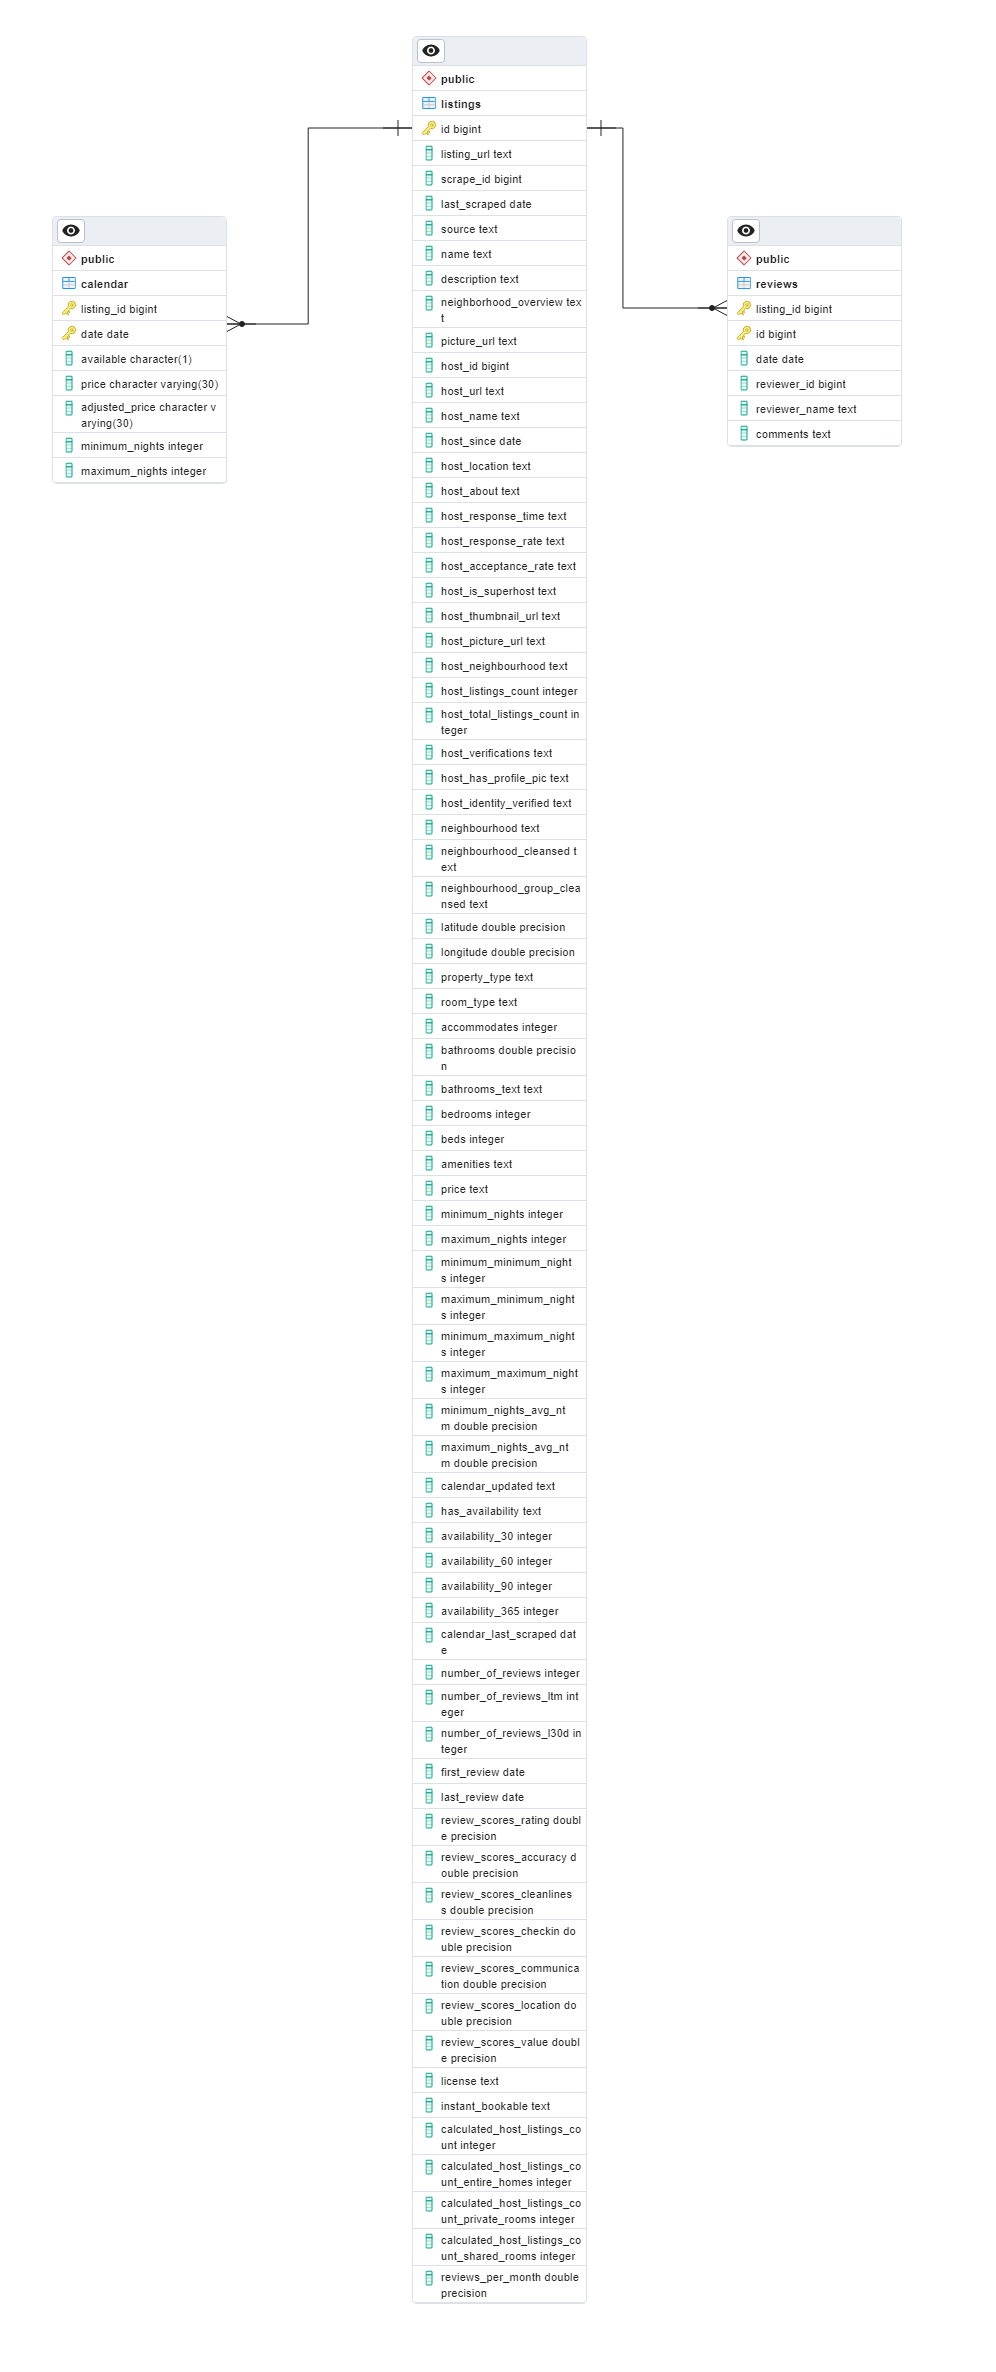
\includegraphics[scale=0.24]{capturas/Schema.png}
    \caption{Esquema Entidad/Relación de la base de datos.}
    \label{fig:esquema-bd}
\end{figure}

\newpage
\subsection*{Explicación de los datos: tabla 'listings'}

\begin{itemize}[topsep=0pt, partopsep=0pt, itemsep=0pt, parsep=0pt]
\item \textbf{id}: Identificador único del listado (BIGINT).
\item \textbf{listing$\_$url}: URL del listado (TEXT, no nulo).
\item \textbf{scrape$\_$id}: Identificador de la extracción (BIGINT).
\item \textbf{last$\_$scraped}: Fecha en la que se realizó la última extracción (DATE).
\item \textbf{source}: Fuente del listado (TEXT).
\item \textbf{name}: Nombre del listado (TEXT).
\item \textbf{description}: Descripción del listado (TEXT).
\item \textbf{neighborhood$\_$overview}: Descripción del vecindario (TEXT).
\item \textbf{picture$\_$url}: URL de la imagen del listado (TEXT).
\item \textbf{host$\_$id}: Identificador único del anfitrión (BIGINT, no nulo).
\item \textbf{host$\_$url}: URL del perfil del anfitrión (TEXT, no nulo).
\item \textbf{host$\_$name}: Nombre del anfitrión (TEXT).
\item \textbf{host$\_$since}: Fecha en la que el anfitrión se unió (DATE).
\item \textbf{host$\_$location}: Ubicación del anfitrión (TEXT).
\item \textbf{host$\_$about}: Descripción del anfitrión (TEXT).
\item \textbf{host$\_$response$\_$time}: Tiempo de respuesta del anfitrión (TEXT).
\item \textbf{host$\_$response$\_$rate}: Tasa de respuesta del anfitrión (TEXT).
\item \textbf{host$\_$acceptance$\_$rate}: Tasa de aceptación del anfitrión (TEXT).
\item \textbf{host$\_$is$\_$superhost}: Indica si el anfitrión es un superhost (TEXT).
\item \textbf{host$\_$thumbnail$\_$url}: URL de la imagen en miniatura del anfitrión (TEXT).
\item \textbf{host$\_$picture$\_$url}: URL de la imagen del anfitrión (TEXT).
\item \textbf{host$\_$neighbourhood}: Vecindario del anfitrión (TEXT).
\item \textbf{host$\_$listings$\_$count}: Número de listados del anfitrión (INTEGER).
\item \textbf{host$\_$total$\_$listings$\_$count}: Número total de listados del anfitrión (INTEGER).
\item \textbf{host$\_$verifications}: Métodos de verificación del anfitrión (TEXT).
\item \textbf{host$\_$has$\_$profile$\_$pic}: Indica si el anfitrión tiene una foto de perfil (TEXT).
\item \textbf{host$\_$identity$\_$verified}: Indica si la identidad del anfitrión ha sido verificada (TEXT).
\item \textbf{neighbourhood}: Nombre del vecindario (TEXT).
\item \textbf{neighbourhood$\_$cleansed}: Nombre del vecindario (limpiado) (TEXT).
\item \textbf{neighbourhood$\_$group$\_$cleansed}: Nombre del grupo de vecindarios (limpiado) (TEXT).
\item \textbf{latitude}: Latitud de la ubicación del listado (FLOAT).
\item \textbf{longitude}: Longitud de la ubicación del listado (FLOAT).
\item \textbf{property$\_$type}: Tipo de propiedad (TEXT).
\item \textbf{room$\_$type}: Tipo de habitación (TEXT).
\item \textbf{accommodates}: Capacidad de alojamiento (INTEGER).
\item \textbf{bathrooms}: Número de baños (FLOAT).
\item \textbf{bathrooms$\_$text}: Descripción de los baños (TEXT).
\item \textbf{bedrooms}: Número de dormitorios (INTEGER).
\item \textbf{beds}: Número de camas (INTEGER).
\item \textbf{amenities}: Comodidades del listado (TEXT).
\item \textbf{price}: Precio del listado (TEXT).
\item \textbf{minimum$\_$nights}: Número mínimo de noches para reservar (INTEGER).
\item \textbf{maximum$\_$nights}: Número máximo de noches para reservar (INTEGER).
\item \textbf{minimum$\_$minimum$\_$nights}: Número mínimo de noches requeridas en la reserva más restrictiva (INTEGER).
\item \textbf{maximum$\_$minimum$\_$nights}: Número máximo de noches requeridas en la reserva más restrictiva (INTEGER).
\item \textbf{minimum$\_$maximum$\_$nights}: Número mínimo de noches permitidas en la reserva más permisiva (INTEGER).
\item \textbf{maximum$\_$maximum$\_$nights}: Número máximo de noches permitidas en la reserva más permisiva (INTEGER).
\item \textbf{minimum$\_$nights$\_$avg$\_$ntm}: Promedio mínimo de noches requeridas para reservar (FLOAT).
\item \textbf{maximum$\_$nights$\_$avg$\_$ntm}: Promedio máximo de noches requeridas para reservar (FLOAT).
\item \textbf{calendar$\_$updated}: Fecha de actualización del calendario (TEXT).
\item \textbf{has$\_$availability}: Indica si hay disponibilidad (TEXT).
\item \textbf{availability$\_$30}: Número de días de disponibilidad en los próximos 30 días (INTEGER).
\item \textbf{availability$\_$60}: Número de días de disponibilidad en los próximos 60 días (INTEGER).
\item \textbf{availability$\_$90}: Número de días de disponibilidad en los próximos 90 días (INTEGER).
\item \textbf{availability$\_$365}: Número de días de disponibilidad en los próximos 365 días (INTEGER).
\item \textbf{calendar$\_$last$\_$scraped}: Fecha en la que se realizó la última extracción del calendario (DATE).
\item \textbf{number$\_$of$\_$reviews}: Número total de reseñas (INTEGER).
\item \textbf{number$\_$of$\_$reviews$\_$ltm}: Número de reseñas en los últimos 12 meses (INTEGER).
\item \textbf{number$\_$of$\_$reviews$\_$l30d}: Número de reseñas en los últimos 30 días (INTEGER).
\item \textbf{first$\_$review}: Fecha de la primera reseña (DATE).
\item \textbf{last$\_$review}: Fecha de la última reseña (DATE).
\item \textbf{review$\_$scores$\_$rating}: Puntuación de las reseñas (FLOAT).
\item \textbf{review$\_$scores$\_$accuracy}: Puntuación de precisión en las reseñas (FLOAT).
\item \textbf{review$\_$scores$\_$cleanliness}: Puntuación de limpieza en las reseñas (FLOAT).
\item \textbf{review$\_$scores$\_$checkin}: Puntuación de check-in en las reseñas (FLOAT).
\item \textbf{review$\_$scores$\_$communication}: Puntuación de comunicación en las reseñas (FLOAT).
\item \textbf{review$\_$scores$\_$location}: Puntuación de ubicación en las reseñas (FLOAT).
\item \textbf{review$\_$scores$\_$value}: Puntuación de valor en las reseñas (FLOAT).
\item \textbf{license}: Licencia relacionada con el listado (TEXT).
\item \textbf{instant$\_$bookable}: Indica si el listado se puede reservar de forma instantánea (TEXT).
\item \textbf{calculated$\_$host$\_$listings$\_$count}: Número de listados calculados para el anfitrión (INTEGER).
\item \textbf{calculated$\_$host$\_$listings$\_$count$\_$entire$\_$homes}: Número de listados calculados para el anfitrión que son hogares completos (INTEGER).
\item \textbf{calculated$\_$host$\_$listings$\_$count$\_$private$\_$rooms}: Número de listados calculados para el anfitrión que son habitaciones privadas (INTEGER).
\item \textbf{calculated$\_$host$\_$listings$\_$count$\_$shared$\_$rooms}: Número de listados calculados para el anfitrión que son habitaciones compartidas (INTEGER).
\item \textbf{reviews$\_$per$\_$month}: Número de reseñas promedio por mes (FLOAT).
\end{itemize}
\subsection*{Explicación de los datos: tabla 'reviews'}

\begin{itemize}[topsep=0pt, partopsep=0pt, itemsep=0pt, parsep=0pt]
\item \textbf{listing$\_$id}: Identificador del listado (BIGINT).
\item \textbf{id}: Identificador único de la reseña (BIGINT).
\item \textbf{date}: Fecha de la reseña (DATE).
\item \textbf{reviewer$\_$id}: Identificador del revisor (BIGINT).
\item \textbf{reviewer$\_$name}: Nombre del revisor (TEXT).
\item \textbf{comments}: Comentarios de la reseña (TEXT).
\end{itemize}

\subsection*{Explicación de los datos: tabla 'calendar'}
\begin{itemize}[topsep=0pt, partopsep=0pt, itemsep=0pt, parsep=0pt]
\item \textbf{listing$\_$id}: Identificador del listado (BIGINT).
\item \textbf{date}: Fecha del calendario (DATE).
\item \textbf{available}: Indicador de disponibilidad (CHAR(1)).
\item \textbf{price}: Precio (VARCHAR(30)).
\item \textbf{adjusted$\_$price}: Precio ajustado (VARCHAR(30)).
\item \textbf{minimum$\_$nights}: Número mínimo de noches (INTEGER).
\item \textbf{maximum$\_$nights}: Número máximo de noches (INTEGER).
\end{itemize}

\newpage
\subsection*{Manejo de los datos}
\begin{enumerate}
    \item \textbf{Clave primaria:} La clave primaria identifica de manera única cada registro en una tabla.
    \begin{itemize}
        \item Para la tabla "listings", se ha seleccionado el atributo "id" como clave primaria de tipo \texttt{BIGINT}. El atributo "id" proporciona un identificador único para cada registro de la tabla y permite la indexación eficiente y la recuperación rápida de datos.

        \item En las tablas "reviews" y "calendar", se ha utilizado una combinación de atributos ("$listing_id$" e "id" en "reviews" y "$listing_id$" y "date" en "calendar") como clave primaria compuesta para garantizar la unicidad de los registros.
    \end{itemize}
    \item \textbf{Clave foránea:} Las claves foráneas aseguran la integridad referencial y permiten realizar consultas y operaciones que involucren datos relacionados en las diferentes tablas. Se ha establecido una relación entre las tablas "reviews" y "calendar" con la tabla "listings" mediante el uso de claves foráneas. 
    \begin{itemize}
        \item En la tabla "reviews", el atributo "$listing_id$" se utiliza como clave foránea que referencia el atributo "id" de la tabla "listings".

        \item De manera similar, en la tabla "calendar", el atributo "$listing_id$" se utiliza como clave foránea que referencia el atributo "id" de la tabla "listings".
    \end{itemize}
    
    \item \textbf{Tipos de datos:} Se han elegido tipos de datos adecuados para cada atributo en función de la naturaleza de los datos que se almacenan. Por ejemplo:
    \begin{itemize}
        \item Los atributos que almacenan texto largo, como descripciones y comentarios, se han definido como tipo \texttt{TEXT} para permitir una capacidad de almacenamiento más amplia.

        \item Los identificadores y conteos, como "id", "$host_id$" y "$number_of_reviews$", se han seleccionado como tipo \texttt{BIGINT} para manejar valores enteros grandes.

        \item Los datos de fecha se han definido como tipo \texttt{DATE} para almacenar información sobre fechas específicas.

        \item Los precios se han definido como tipo \texttt{TEXT} o \texttt{VARCHAR(30)} para permitir la representación de diferentes formatos y monedas.
    \end{itemize}

\end{enumerate}